%%% final.tex
%%%
%%% This LaTeX source document can be used as the basis for your technical
%%% paper or abstract. Intentionally stripped of annotation, the parameters
%%% and commands should be adjusted for your particular paper - title, 
%%% author, article DOI, etc.
%%% The accompanying ``template.annotated.tex'' provides copious annotation
%%% for the commands and parameters found in the source document. (The code
%%% is identical in ``template.tex'' and ``template.annotated.tex.'')

\documentclass[conference]{acmsiggraph}

\usepackage{amsmath}
\usepackage{amssymb}
\TOGonlineid{45678}
\TOGvolume{0}
\TOGnumber{0}
\TOGarticleDOI{1111111.2222222}
\TOGprojectURL{}
\TOGvideoURL{}
\TOGdataURL{}
\TOGcodeURL{}

\title{Rendering Metaballs with PBRT}

\author{Vinícius Vendramini\thanks{e-mail:todo@email.com}\\IME-USP \and Wilson K. Mizutani\thanks{e-mail:kazuo@ime.usp.br}\\IME-USP}
\pdfauthor{Vinícius Vendramini, Wilson K. Mizutani}

\keywords{implicit surface, metaball, mesh generation, ray tracing}

\begin{document}

%% \teaser{
%%   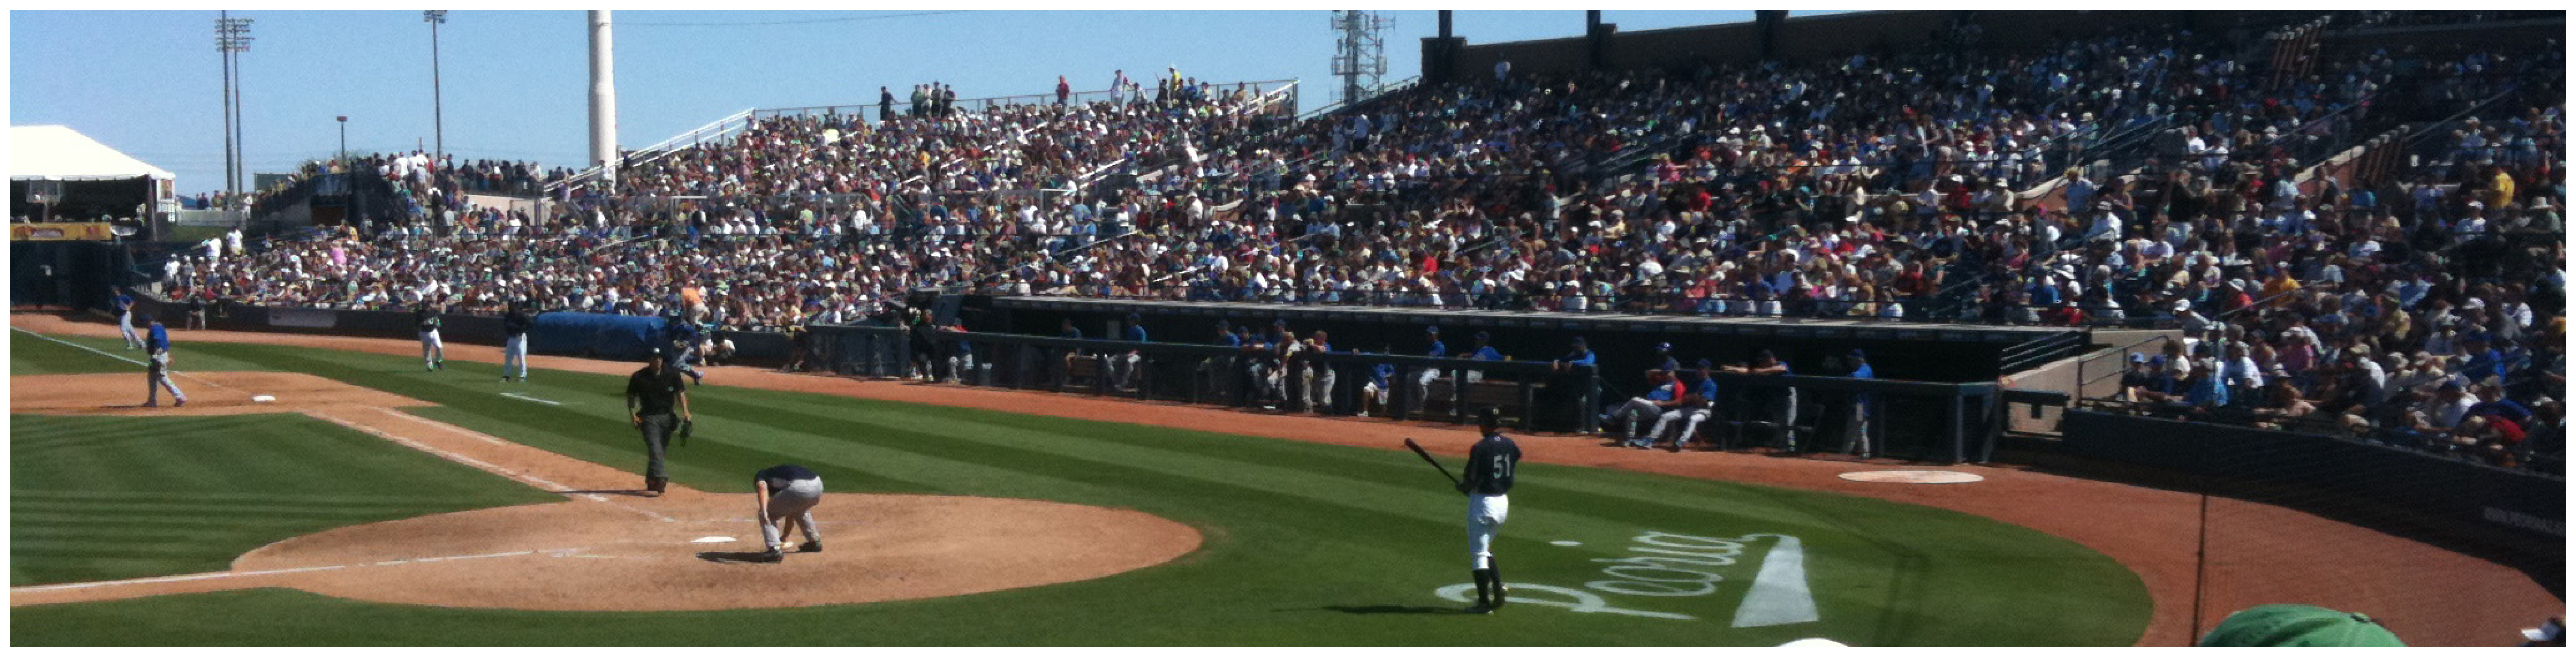
\includegraphics[height=1.5in]{images/sampleteaser}
%%   \caption{Spring Training 2009, Peoria, AZ.}
%% }

\maketitle

\begin{abstract}

Three dimensional geometry is often made through meshes, which requires
either modeling skills or data extraction from real bodies. This is specially
difficult for more organic or fluid structures, like creatures, liquids or
gases. Blinn \shortcite{Blinn:1982:GAS:965145.801290} proposes a way of defining
geometry through a particular type of implicit surface that provides a simple
way of representing such geometries. These surfaces are also known as
\textit{metaballs}). In this work we strive for a thourough renderization of
these geometries using the highly awarded PBRT
\shortcite{Pharr:2010:PBR:1854996} render system. There are two methods covered:
one based on Blinn's original intersection algorithm, and another using the
marching cubes algorithm \cite{Lorensen:1987:MCH:37402.37422} to generate a mesh
that approximates the surface.

\end{abstract}

%\begin{CRcatlist}
%  \CRcat{I.3.3}{Computer Graphics}{Rendering Metaballs with PBRT}{Implicit surfaces}
%  \CRcat{I.3.7}{Computer Graphics}{Rendering Metaballs with PBRT}{Ray-tracing};
%\end{CRcatlist}

\keywordlist

%% Use this only if you're preparing a technical paper to be published in the 
%% ACM 'Transactions on Graphics' journal.

\TOGlinkslist

%% Required for all content. 

\copyrightspace

\section{Introduction}

There are many physical structures that can be described as being a composition
of bumps or blobs. A cloud, for instance, could be constructed as many smaller,
simpler clouds put together, merging in the regions between them. That is very
similar to what happens with electron densities when molecules form from
individual atoms: the resulting combined electrospheres combine where the atoms
join each other. Other examples could be liquids in general (the bumps would be
individual drops) or even flesh-based creature bodies (the blobs would ``grow''
from the bones). One way of defining this representation is through the use of
\textit{metaballs}, as seen in \cite{Blinn:1982:GAS:965145.801290} (the term
\textit{metaball} was not actually used in the original text).

\subsection{Metaballs}

Blinn \shortcite{Blinn:1982:GAS:965145.801290} defines a particular type of
implicit surface that is a composition of simpler implicit surfaces. An implicit
surface is the set of points in $\mathbb{R}^n$ that solves the equation
$F(x) = 0$ for a given function $F:\mathbb{R}^n \rightarrow \mathbb{R}$. For
example, the function $F(x) = \|x\|^{-1} - 1$ gives an implicit surface
consisting of a hypersphere of radius $1$. The surface Blinn presents defines
this $F$ in $\mathbb{R}^3$ as follows:

\begin{equation}
  F(x) = D(x) - T
\end{equation}

Where $T$ is a \textit{threshold} value (usually $1$) and
$D:\mathbb{R}^3 \rightarrow \mathbb{R}$ is the sum of $n$ exponentials, each
corresponding to an individual bump of the metaball:

\begin{equation}
  D(x) = \sum_{i=1}^{n} b_i e^{-a_i \|x-P_i\|}
\end{equation}

Where $P\in\mathbb{R}^3$ and $b_i,a_i\in\mathbb{R}$ for $i=1,...,n$. The
exponentials also represent spheres, with $P_i$ being their respective centers
and $a_i$ and $b_i$ factors that together determine the radius and how much each
bump clings to each other. Since these two coefficients are not very intuitive,
Blinn proposes a few change of variables, aswell as using the squared distance
$\|x-P_i\|^2$ for code optimization. The resulting formula is:

\begin{equation}
  D(x) = \sum_{i=1}^{n} T e^{\frac{B_i}{R_i^2}\|x-P_i\|^2 - B_i}
\end{equation}

In this version, $R_i$ is the bump's radius, and $B_i$ is its blobbiness
factor, which must be negative. The closer to zero the blobbiness factor is,
the more merged and homogeneous neighbouring bumps become. Also, it is assumed
that $T=1$ in this form.

With the metaball representation, it is possible to build very complex fluid
geometries by simply placing various bumps (with possibly varying radiuses and
blobbiness) and using an aproppriate material, as seen in Figure
\ref{img:metaball-liquid}\footnotemark{}.

Another very important property of implicit surfaces in general, is that if
$F(x)$ is differentiable, then a nonzero gradient $\nabla F$ at a point $x$ is
the surface normal at that point, towards the growing size. In the case of
Blinn's metaballs, the gradient gives an inwards normal, so for shading
purposes, $-\nabla F(x)$ is used.

\begin{figure}[ht]
  \centering
  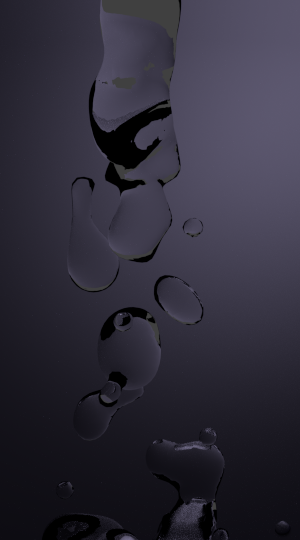
\includegraphics[width=1.5in]{images/fluid.png}
  \caption{Renderization of a liquid with metaballs.}
  \label{img:metaball-liquid}
\end{figure}

\footnotetext{
  This rendered image was made using the Blender Cycles Engine software with
  particle fluid simulation \cite{Blender}
}

\subsection{PBRT}

\subsection{Rendering methods}


\section{Marching cubes algorithm}

The marching cubes algorithm was introduced by Lorensen and Cline in 87 as an efficient way to render isosurfaces. The algorithm uses a divide-and-conquer approach by dividing the space that contains the surface into several much smaller cubes and then analysing the way the surface intersects with each cube. The nature of isosurfaces makes it easy to determine if each vertex is on one side or the other of any given cube. Based on the set of vertices that are on one side (ie the inside), the algorithm uses a preprocessed table containing several possible triangulations of the cubes to find the better triangular approximation to the piece of the isosurface contained within that cube. The way the triagulations are chosen guarantees the resulting surface will be topologically correct, even in the complicated ambiguous cases. 






\subsection{Ambiguous cases}

\begin{equation}
 \sum_{j=1}^{z} j = \frac{z(z+1)}{2}
\end{equation}

\begin{eqnarray}
x & \ll & y_{1} + \cdots + y_{n} \\
  & \leq & z
\end{eqnarray}

\section{Analytic intersection}


\begin{figure}[ht]
  \centering
  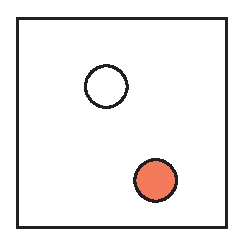
\includegraphics[width=1.5in]{images/samplefigure}
  \caption{Sample illustration.}
\end{figure}

\section{Implmentation}

\subsection{Marching cubes}

\subsection{Intersection}

\section{Conclusion}

Lorem ipsum dolor sit amet, consectetur adipisicing elit, sed do
eiusmod tempor incididunt ut labore et dolore magna aliqua. Ut enim ad
minim veniam, quis nostrud exercitation ullamco laboris nisi ut
aliquip ex ea commodo consequat. Duis aute irure dolor in
reprehenderit in voluptate velit esse cillum dolore eu fugiat nulla
pariatur. Excepteur sint occaecat cupidatat non proident, sunt in
culpa qui officia deserunt mollit anim id est laborum.

\subsection{Future works}

\section*{Acknowledgements}

%TODO

\bibliographystyle{acmsiggraph}
\bibliography{template}
\end{document}
